% !TeX spellcheck = de_DE
\documentclass{uebung_cs}
\usepackage{algo121}
\blattname{Wochenplan: Disjunkte Mengen, Union-Find}

%%%%%%%%%%%%%%%%%%%%%%%%%%%%%%%%%%%%%%%%%%%%%%%%%%%%%%%%%%%%%%%%%%%%%%%%%%%%

\newboolean{programming}
\setboolean{programming}{false}

%%%%%%%%%%%%%%%%%%%%%%%%%%%%%%%%%%%%%%%%%%%%%%%%%%%%%%%%%%%%%%%%%%%%%%%%%%%%
% Makros für noch nicht übersetzte Begrifflichkeiten
\newcommand{\qfind}{\textit{\textbf{Quick Find}}}
\newcommand{\qunion}{\textit{\textbf{Quick Union}}}
\newcommand{\wqunion}{\textit{\textbf{Weighted Quick Union}}}
\newcommand{\pathcomp}{\textit{\textbf{Path Compression}}}


\begin{document}
\section*{Vorbereitung}
Lies E Kapitel 8 ohne 8.7 (oder CLRS Kapitel 24 ohne 24.1 und 24.4) und schau das Video der Woche.

\section*{Dienstag}
\begin{aufgabe}[Algorithmen und Eigenschaften]\label{tue-first}
	\begin{enumerate}
		\item (\warmup) Gegeben sei der Graph aus Abbildung 1.
		Zeige den Baum der kürzesten Wege für den Graphen (Startknoten 0).
		Schreibe die Länge des kürzesten Weges von Knoten 0 zu jedem Knoten.
		\item Gib einen Beispiel-Graphen mit negativen Kanten, aber ohne negative Kreise, der für eine falsche Ausgabe des Dijkstra Algorithmus sorgt.
		\item Gegeben sei nun ein Graph $G$ mit $n$ Knoten und $m$ Kanten, und ein Baum $T$ in $G$ mit Wurzel in Knoten $s$.
		Zeige, wie man in $\O (n+m)$ feststellt, ob $T$ der Baum der kürzesten Wege mit Startknoten $s$ ist.
		\item Sei $T$ der Baum der kürzesten Wege von Knoten $s$ in Graph $G$.
		Ist $T$ immer noch der Baum der kürzesten Wege, wenn wir auf alle Kantengewichte eine Konstante $c$ addieren?
	\end{enumerate}
\end{aufgabe}

\begin{aufgabe}[Noch mehr Kabel]
	Die Kabelfernsehen-Firma AlgoMedia überträgt Kabelfernsehen an alle Häuser in Algo-Stadt.
	Sie übermitteln die TV Signale von ihrem Hauptsitz mittels eines Kabelnetzwerks, wobei die Länge jedes Kabels bekannt ist.
	Die Kabel verlaufen zwischen einer Menge an Boxen.
	Es gibt eine Box in jedem Haus, eine in dem Hauptsitz und sonst keine weiteren Boxen.
	Jede Box kann mit mehreren Kabeln verbunden werden. Es gibt $X$ Häuser und $K$ Kabel im Netzwerk.\\
	Löse folgende Aufgaben:
	\begin{enumerate}
		\item AlgoMedia möchte, dass alle Kund:innen das bestmögliche Signal erhalten.
		Die Signalqualität sinkt proportional zur Länge des Kabels.
		Gib einen Algorithmus zur Bestimmung der besten Möglichkeit für die Signalstrecken zur Maximierung der Qualität an.
		\item Nach genauerer Betrachtung bemerkt AlgoMedia, dass die Qualität eines Signals, wenn es durch eine Box geht so sinkt, wie bei 5 Metern Kabellänge.
		Gib einen Algorithmus zur Bestimmung der besten Möglichkeit für die Signalstrecken zur Maximierung der Qualität in diesem Szenario an.
		\item Nach Kürzungen bei staatlichen Mitteln versucht AlgoMedia Geld zu sparen.
		Aktuell geben sie 42.000 Euro im Jahr für ein Meter Kabel aus.
		Gib einen Algorithmus zur Bestimmung der günstigsten Möglichkeit, um alle Häuser in Algo-Stadt mit einem Signal zu versorgen.
	\end{enumerate}
\end{aufgabe}


\begin{aufgabe}[Längster Pfad in gerichteten azyklischen Graphen]
	Bestimme einen Algorithmus, um den längsten Weg in einem gerichteten, kreisfreien Graphen zu finden.
\end{aufgabe}

\begin{aufgabe}[Dijkstra und die Knotengewichte]
	Sei $G$ ein gerichteter Graph bei dem alle Knoten ein nicht-negatives Gewicht haben.
	Das Gewicht eines Weges in $G$ ist die Summe der Gewichte der Knoten auf dem Weg.
	Bestimme einen Algorithmus, um den kürzesten Weg zwischen zwei Knoten in $G$ zu bestimmen.
\end{aufgabe}

\begin{aufgabe}[Reiseplanung in Zombie-Zeiten, \hard]
	Scheinbar hat deine Gruppe es geschafft der brenzligen Zombiesituation des Union-Find Blattes zu entkommen.
	Jetzt müsst ihr den sichersten Weg zwischen zwei Städten finden, um hoffentlich nicht von Zombies gegessen zu werden.
	Der Graph $G$, in dem jeder Knoten eine Stadt und jede Kante eine Straße zwischen zwei Städten. Für jede Kante $e$ gibt es eine Wahrscheinlichkeit $s(e), 0 \leq s(e) \leq 1$, die angibt, ob man das überqueren der Straße überlebt.
	Die Wahrscheinlichkeiten für die Kanten sind unabhängig und die Wahrscheinlichkeit, auf einem Pfad $P$ zu überleben ist das Produkt über die Wahrscheinlichkeiten der einzelnen Kanten/Straßen.
	\begin{center}
	\scalebox{0.8}{
	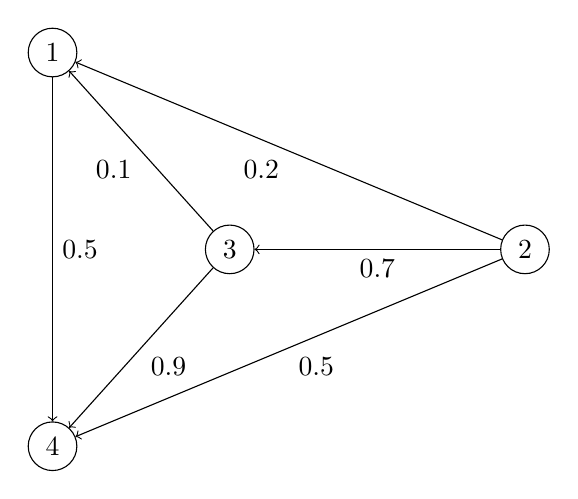
\begin{tikzpicture}[->, auto]
		\tikzstyle{vertex} = [circle, draw]
		\node[vertex](A) at (0,5) {1};
		\node[vertex](B) at (2.25,2.5) {3};
		\node[vertex](C) at (6,2.5) {2};
		\node[vertex](D) at (0,0) {4};
		\path  (B) edge node {0.1} (A);
		\path  (B) edge node {0.9} (D);
		\path  (C) edge node {0.7} (B);
		\path  (C) edge node {0.5} (D);
		\path  (C) edge node {0.2} (A);
		\path  (A) edge node {0.5} (D);
	\end{tikzpicture}
	}
	\end{center}
	Der obige Graph ist ein Beispielgraph.
	Wenn man direkt von Knoten 2 zu Knoten 4 geht, hat man eine 50\% Chance zu überleben.
	Wenn man aber die Route $2\rightarrow 3 \rightarrow 4$ nimmt, hat man eine $0.7\cdot 0.9 = 0.63 = 63\%$ Chance zu überleben.
	Entwirf einen Algorithmus, der den sichersten Weg zwischen zwei Knoten $s$ und $t$ für einen beliebigen Eingabegraphen bestimmt.
\end{aufgabe}


\begin{aufgabe}[Tiefhängende Äste]
	Eine Weide ist ein gewichteter, gerichteter Graph, der aus einem Binärbaum erstellt wird, indem man für jedes Blatt jeweils eine zur Wurzel gerichtete Kante einfügt.
	Alle Kanten haben nicht-negative Gewichte.
	% Hier tikz Zaubereien
	Betrachte eine Weide mit $n$ Knoten.
	Wir wollen für einen gegebenen Knoten $s$ die kürzesten Wege zu allen anderen Knoten ermitteln.
	\begin{enumerate}
		\item Wie lange braucht der Dijkstra Algorithmus um dieses Problem zu lösen?
		Gib die Laufzeit im Verhältnis zu $n$ an.
		\item (\hard) Entwirf einen schnelleren Algorithmus. 
	\end{enumerate} 
\end{aufgabe}


\end{document}
